% plotting.tex - to be inserted into the the main report.tex file

\section{Outputting and plotting the results} % explain what the output files look like and how they are plotted
The final array contains the numerical value of the electric potential at each point in the grid as a number of type \emph{double}. The program outputs the value of each point along the y-direction corresponding to an x-value, then moves on to the next x-value and repeats the process. The program writes the value of the potential at each point to a file in the format shown in table \ref{table:potential_data}.

After all y values have been outputted for an x value, the final row is followed by an empty row before the next x value is started. This is done to allow gnuplot to plot three dimensional data. This file is used to plot the potential as a heatmap-styled plot, an example of which can be seen in figure \ref{fig:potentialplot}.

\begin{figure}[h!]
\centering
\setlength\fboxsep{0pt}
\setlength\fboxrule{0.5pt}
\fbox{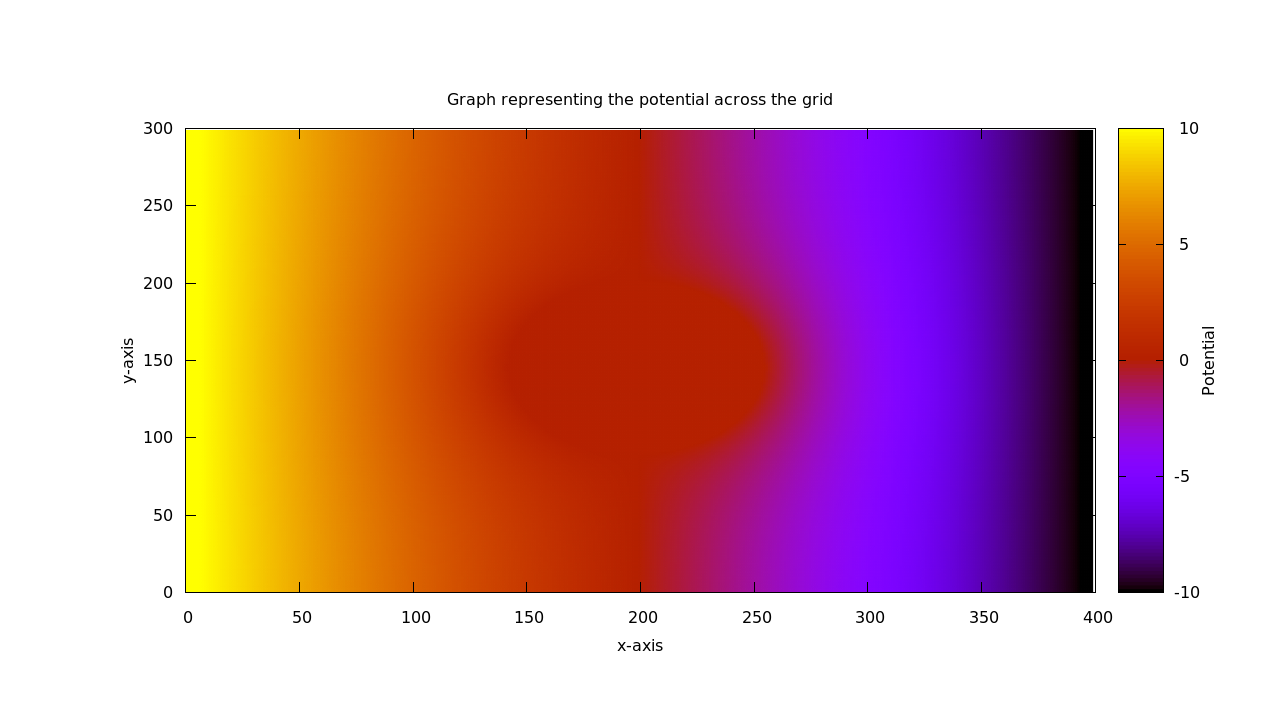
\includegraphics[width=0.95\textwidth, trim = 40mm 20mm 20mm 30mm, clip]{example_potential_plot.png}} % change trim as required to eliminate unnecessary whitespace. trim: left bottom right top
\label{fig:potentialplot}
\caption{A plot representing the electric potential ${\phi}$ at points in the grid.}
\end{figure}

Another output file is also produced to allow the plotting of the electric field. The file contains the x- and y-coordinates as well as the $d{\phi}/dx$ and $d{\phi}/dy$ values, which are approximated. For a point $(x,y)$, the gradient along the x-direction is calculated as the average of the change along one step from the left (-x direction) and one step to the right (+x direction), i.e. $d{\phi}/dx_{x,y} = ( value(x-1,y) - value(x+1,y) ) / 2$. Similarly, for the gradient along the y-direction, the gradient is calculated as the average of the change along one step to the +y direction and one step from the -y direction, i.e. $d{\phi}/dy_{x,y} = ( value(x,y-1) - value(x,y+1) ) / 2$. Here the $\phi$ refers to the potential. The values are written to a file in the format shown in table \ref{table:field_data}.
\begin{table}
    \parbox{0.47\linewidth}{
    \centering
    \begin{tabularx}{0.44\textwidth}{ |XXX| }
        \hline
        $x_1$ & $y_1$ & $value_{1,1}$ \\
        $x_1$ & $y_2$ & $value_{1,2}$ \\
        $x_1$ & $y_3$ & $value_{1,3}$ \\
        & & \\
        $x_2$ & $y_1$ & $value_{2,1}$ \\
        $x_2$ & $y_2$ & $value_{2,2}$ \\
        $x_2$ & $y_3$ & $value_{2,3}$ \\
        & & \\
        $x_3$ & $y_1$ & $value_{3,1}$ \\
        $x_3$ & $y_2$ & $value_{3,2}$ \\
        $x_3$ & $y_3$ & $value_{3,3}$ \\
        \hline
    \end{tabularx}
    \caption{Structure of a file containing information about the potential across the grid. This example is for a 3x3 grid.}
    \label{table:potential_data}
    }
    \hfill
    \parbox{0.47\linewidth}{
    \centering
    \begin{tabularx}{0.44\textwidth}{ |XXXX| }
        \hline
        $x_1$ & $y_1$ & $d{\phi}/dx_{1,1}$ & $d{\phi}/dy_{1,1}$ \\
        $x_1$ & $y_2$ & $d{\phi}/dx_{1,2}$ & $d{\phi}/dy_{1,2}$ \\
        $x_1$ & $y_3$ & $d{\phi}/dx_{1,3}$ & $d{\phi}/dy_{1,3}$ \\
        & & & \\
        $x_2$ & $y_1$ & $d{\phi}/dx_{2,1}$ & $d{\phi}/dy_{2,1}$ \\
        $x_2$ & $y_2$ & $d{\phi}/dx_{2,2}$ & $d{\phi}/dy_{2,2}$ \\
        $x_2$ & $y_3$ & $d{\phi}/dx_{2,3}$ & $d{\phi}/dy_{2,3}$ \\
        & & & \\
        $x_3$ & $y_1$ & $d{\phi}/dx_{3,1}$ & $d{\phi}/dy_{3,1}$ \\
        $x_3$ & $y_2$ & $d{\phi}/dx_{3,2}$ & $d{\phi}/dy_{3,2}$ \\
        $x_3$ & $y_3$ & $d{\phi}/dx_{3,3}$ & $d{\phi}/dy_{3,3}$ \\
        \hline
    \end{tabularx}
    \label{table:field_data}
    \caption{Structure of a file containing information about the electric field across the grid. This example is for a 3x3 grid.}
    }
\end{table}

Again, empty lines are inserted before a change in x-values to make operating gnuplot easier. The data can then be plotted as a vector field in gnuplot using "plot \ldots with vectors". By setting some functions in gnuplot, one can make the vectors in the field of uniform size (to improve readability) and indicate the magnitude of the vector by colour. An example of such a plot can be seen in figure \ref{fig:vectorfieldplot}.

\begin{figure}[h!]
    \centering
    \setlength\fboxsep{0pt}
    \setlength\fboxrule{0.5pt}
    \fbox{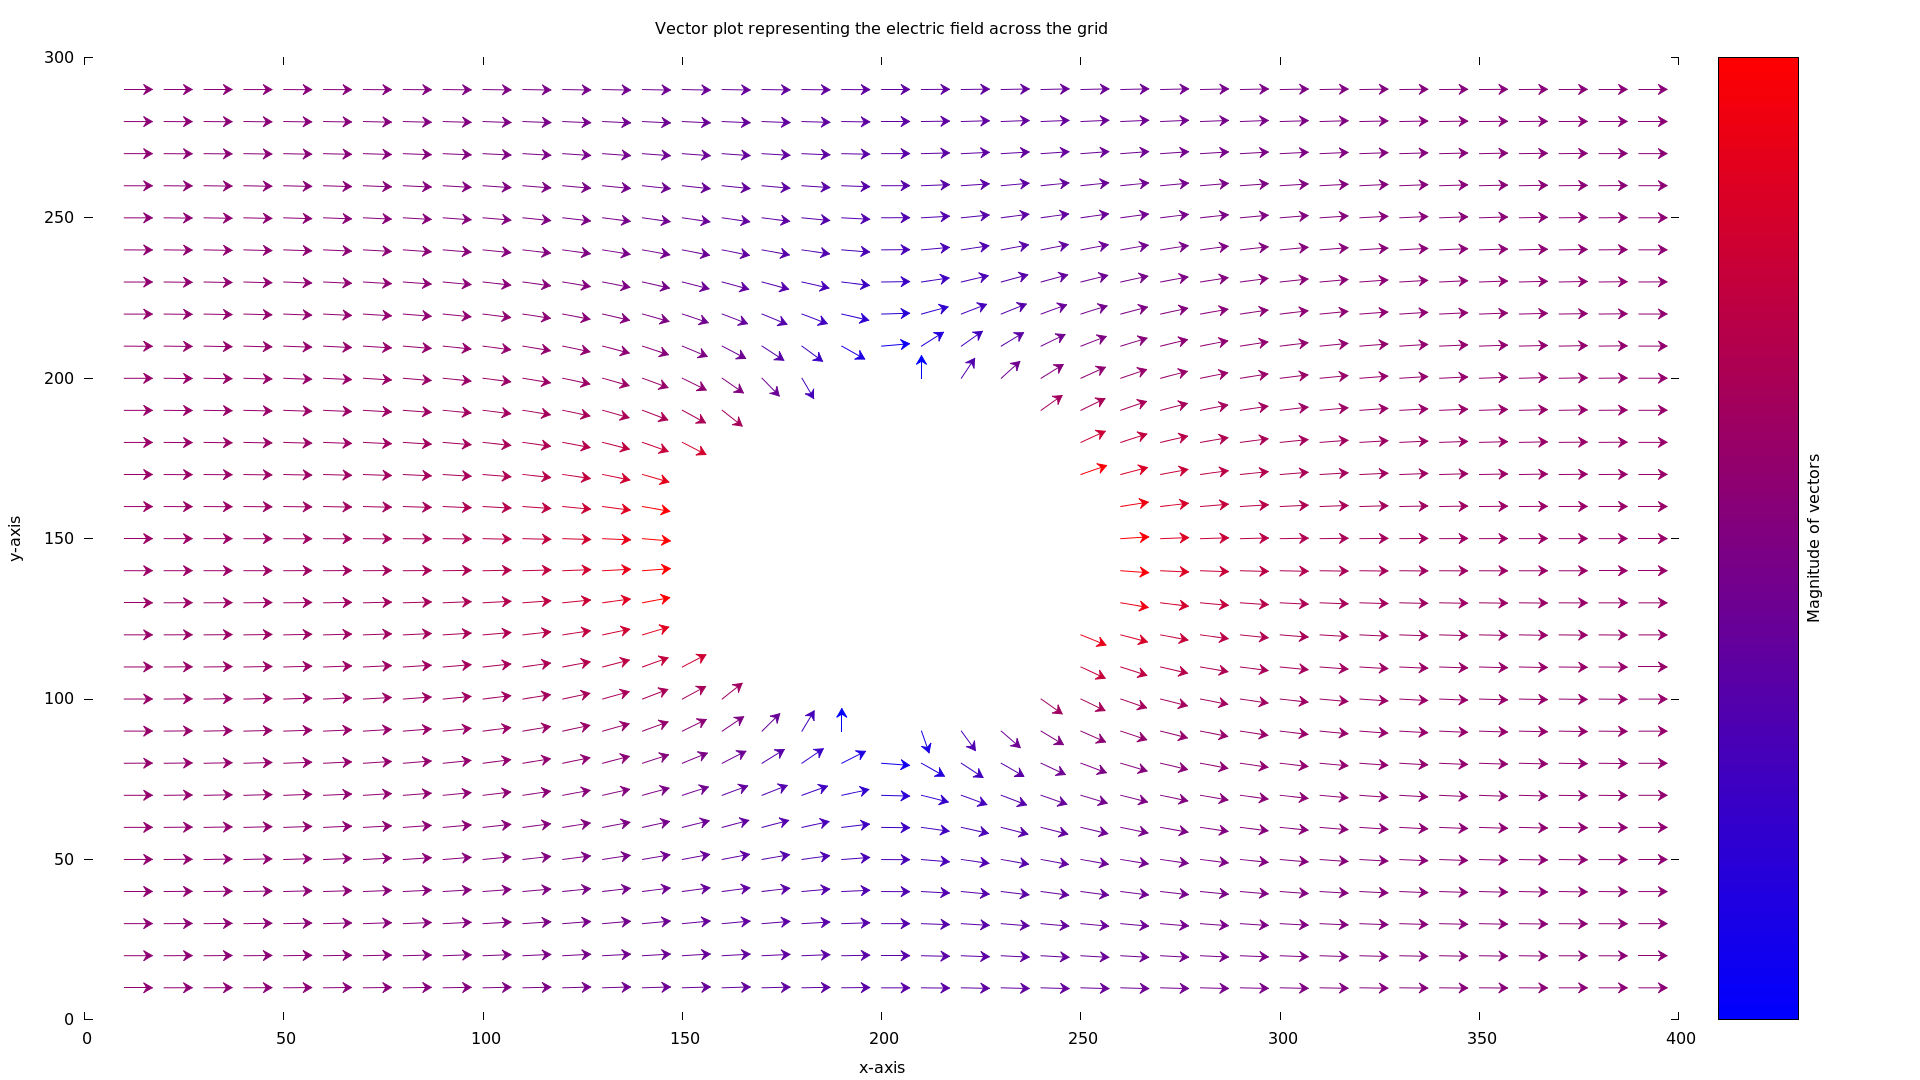
\includegraphics[width=0.95\textwidth, trim = 0mm 0mm 0mm 0mm, clip]{example_vector_field_plot.png}} % trim options: left bottom right top, change to appropriate values if some other image is used and it has too much whitespace around it.
    \caption{A plot representing the electric field calculated for System A, shown as a vector plot with the colour of the vectors indicating the magnitude of the vector: red means large, blue means small.}
    \label{fig:vectorfieldplot}
\end{figure}
 
An equipotential plot is also produced. This uses the same data file as the heatmap-styled plot. The equipotential lines are drawn by the contour function in gnuplot. An example of an equipotential line plot overlaid on a vector field can be seen in figure \ref{fig:vectors_and_contours}.

\begin{figure}[h!]
    \centering
    \setlength\fboxsep{0pt}
    \setlength\fboxrule{0.5pt}
    \fbox{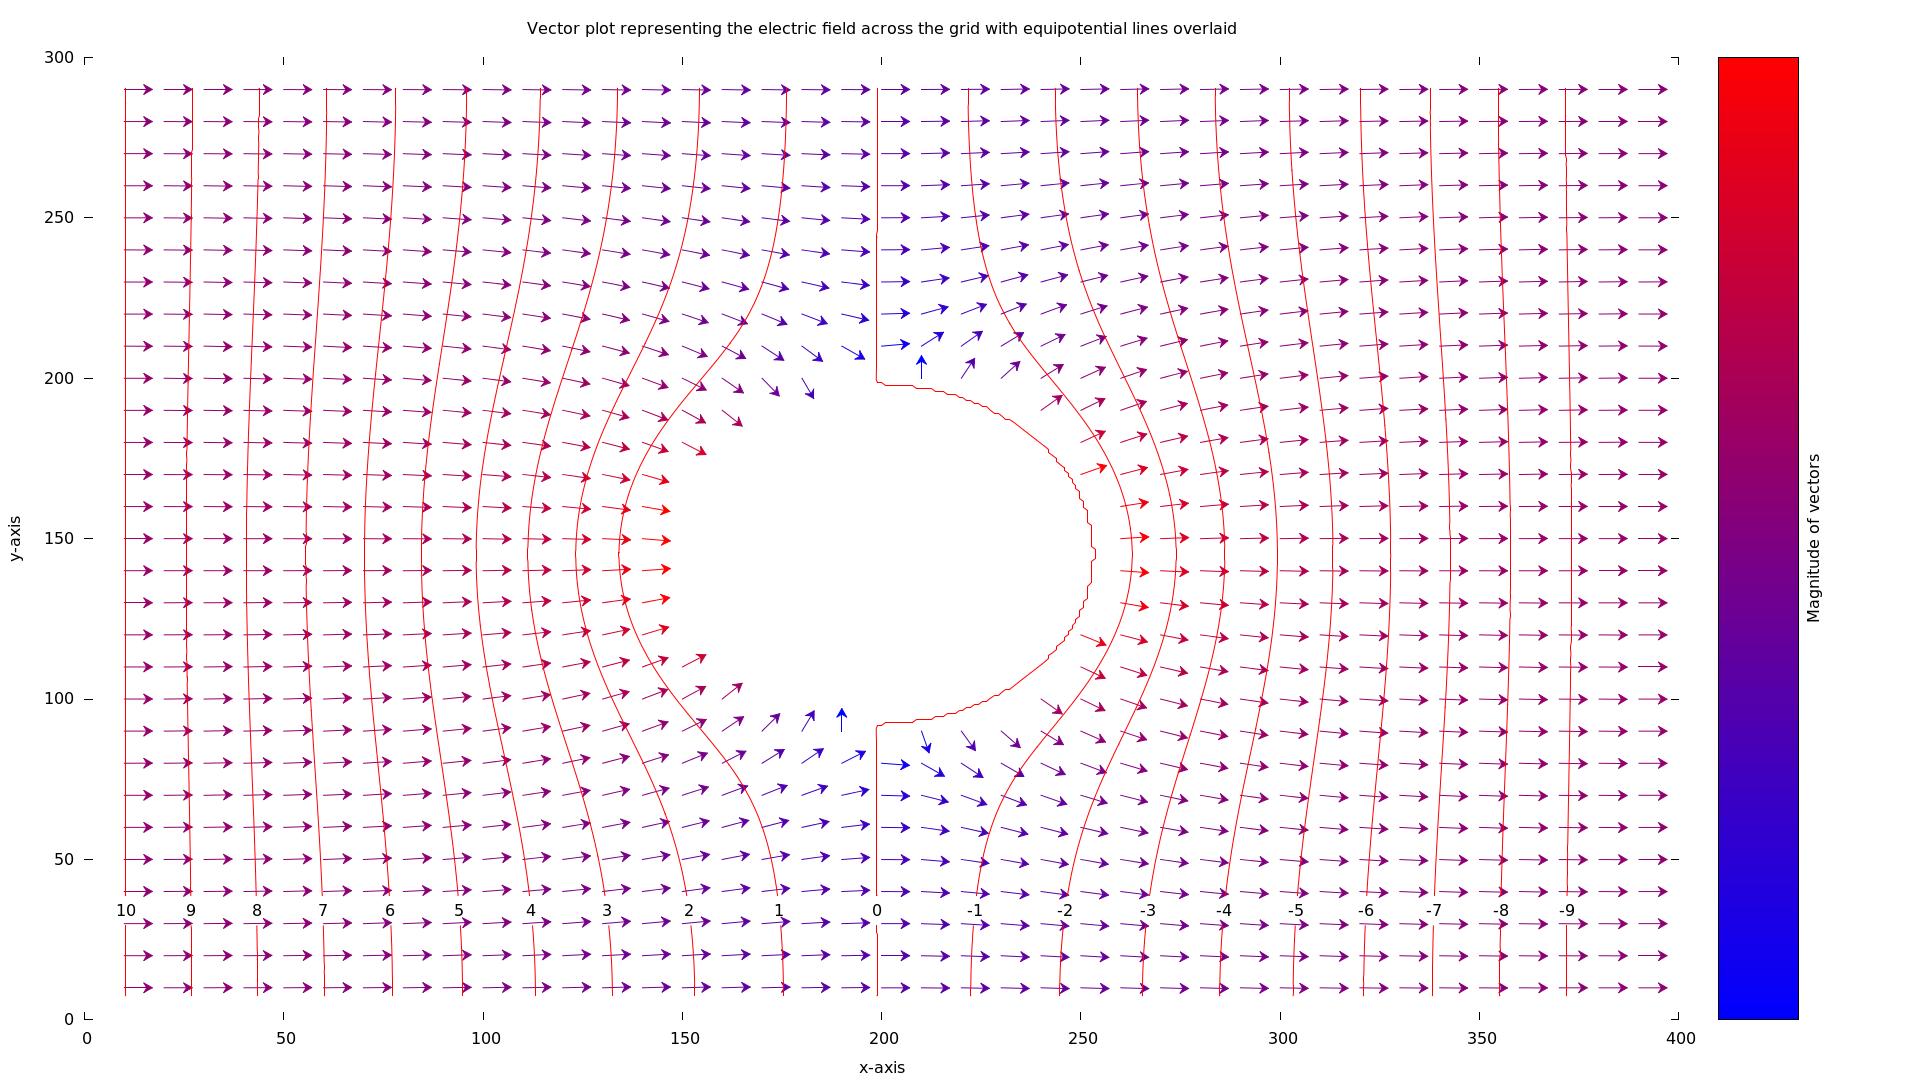
\includegraphics[width=0.95\textwidth, trim = 0mm 0mm 0mm 0mm, clip]{example_vectors_and_contours.png}} % trim options: left bottom right top, change to appropriate values if some other image is used and it has too much whitespace around it.
    \caption{A plot displaying the electric field represented as vectors with equipotential lines overlaid on top of them.}
    \label{fig:vectors_and_contours}
\end{figure}

All of the plotting in the program is done internally via C++ functions which call gnuplot to be run. The source code can be found in the appendix \ref{code:plot.cpp}. % Remove sentence if source code not included.
